\section{Experiments}
\subsection{Tpch SF10}
% To evaluate our memory footpring estimator mechanism we kept each
As a training set for each query, we randomized every selection point and range,
and produced 200 random versions of the query. As a test set we used the original
query.

In query 19 we observe a misprediction of 70\%. The reason this happens, is that
the MAL algebra of this specific query consists of a lot of merge instructions,
for which we output the sum of the two arguments, which in case of merging similar
variables can lead to an almost 2$\times$ overestimation.
This is the basic reason for the large error observed.
\begin{verbatim}
culprit:
C_187 := algebra.thetaselect(X_178, "DELIVER IN PERSON", "==");                                                                                                                                                                                                                    |
X_191 := bat.mergecand(C_187, C_187);                                                                                                                                                                                                                                              |
X_194 := bat.mergecand(X_191, C_187);
\end{verbatim}

The second most deviant query is 16. The dominant reason why there is an 20\%
error is the misprediction of the join instruction(our approach is kNN based).

\begin{figure}[!htb]
  \centering
  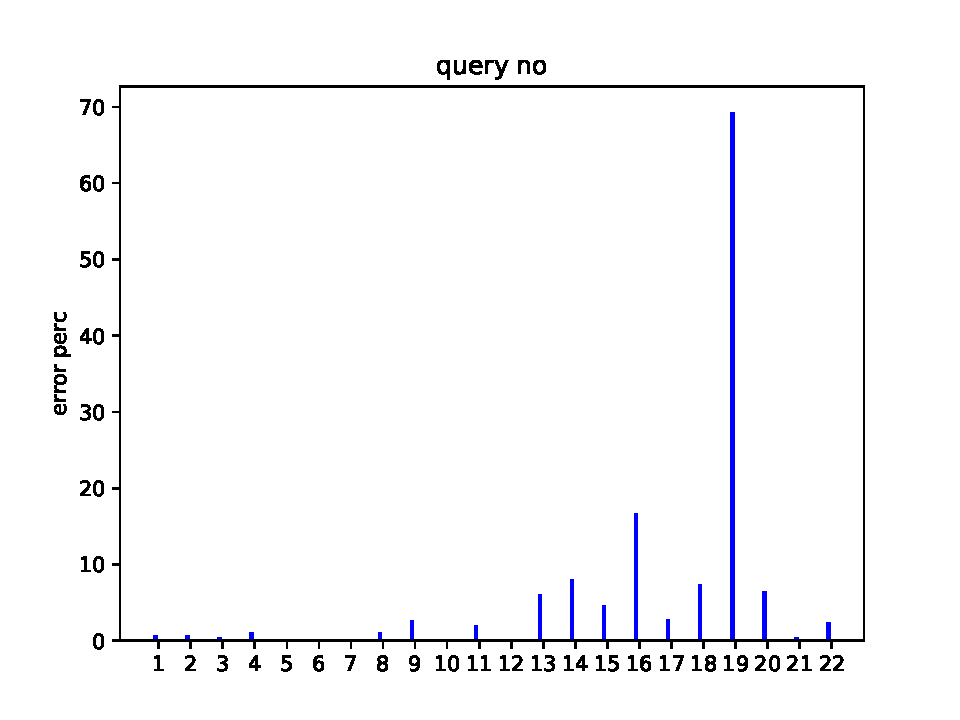
\includegraphics[scale=0.7]{figs/tpch10/mem_error_1-23.pdf}
  \caption{Queries 1-22 memory footprint error}
  \label{fig:tpch10m}
\end{figure}

\subsection{Selection Error }

\subsubsection{Q07}
The selection prediction fails because of a misprediction in the selection
argument count, due to a misprediction in a projectionpath instruction(unknown column)
\subsubsection{Q17}
Argument count misprediction due to a groupdone in an unknown column
\subsubsection{Q18}
The select randomization is weird (having sum > ...)

\begin{figure}[!htb]
  \begin{subfigure}[t]{0.5\textwidth}
    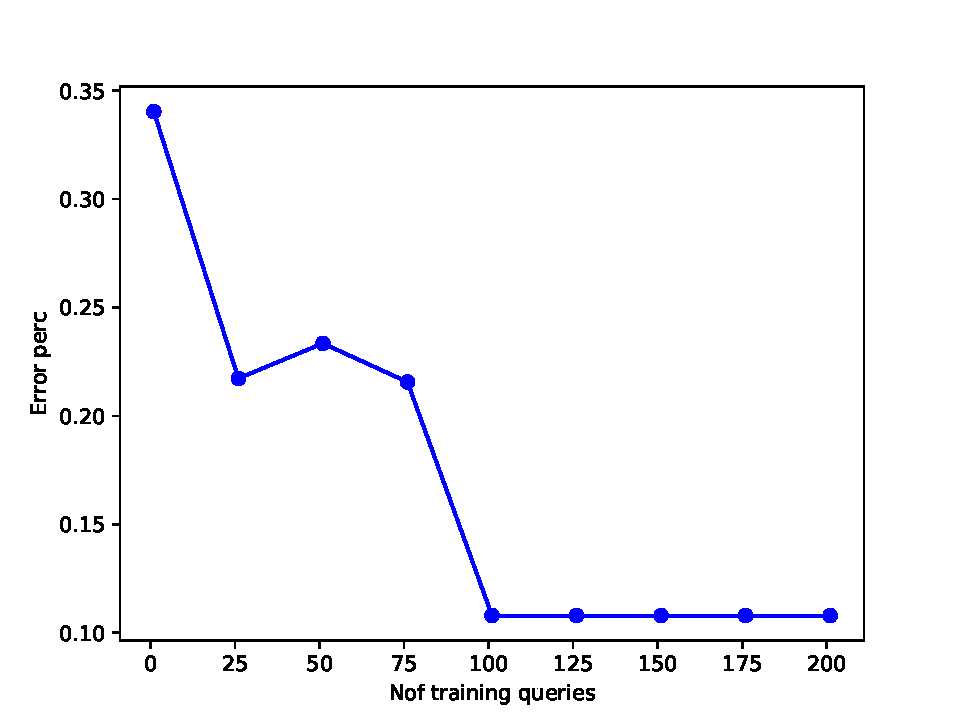
\includegraphics[scale=0.4]{figs/tpch10/tpch10_sel01_error.pdf}
    \caption{Query 01 select error}
    \label{fig:tpch_sel01}
  \end{subfigure}
  \begin{subfigure}[t]{0.5\textwidth}
    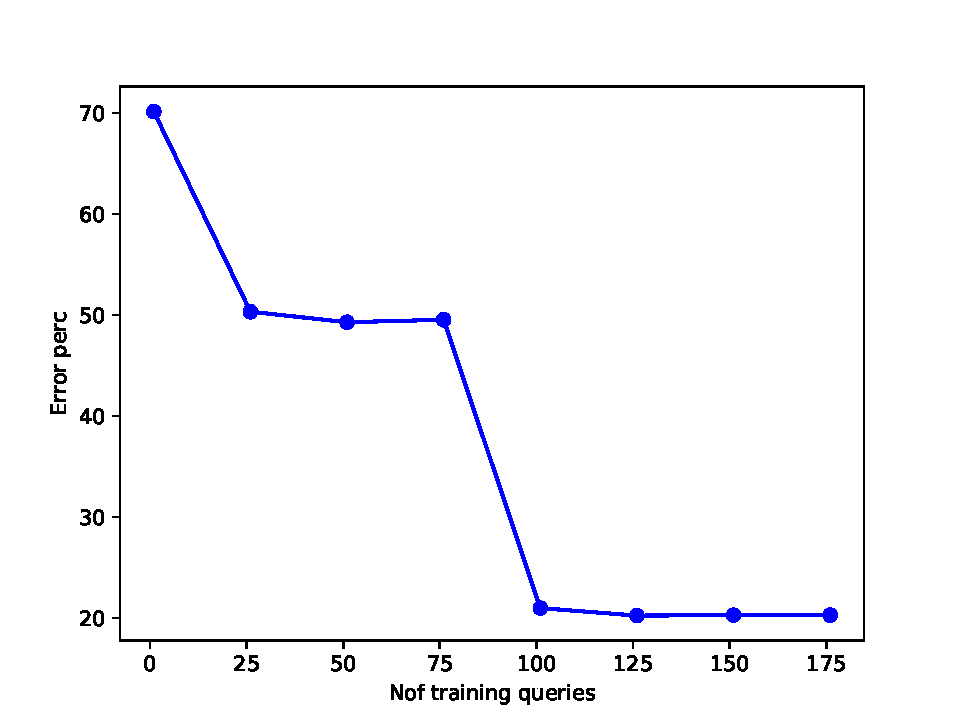
\includegraphics[scale=0.4]{figs/tpch10/tpch10_sel02_error.pdf}
    \caption{Query 02 select error}
    \label{fig:tpch_sel02}
   \end{subfigure}

   \begin{subfigure}[t]{0.5\textwidth}
     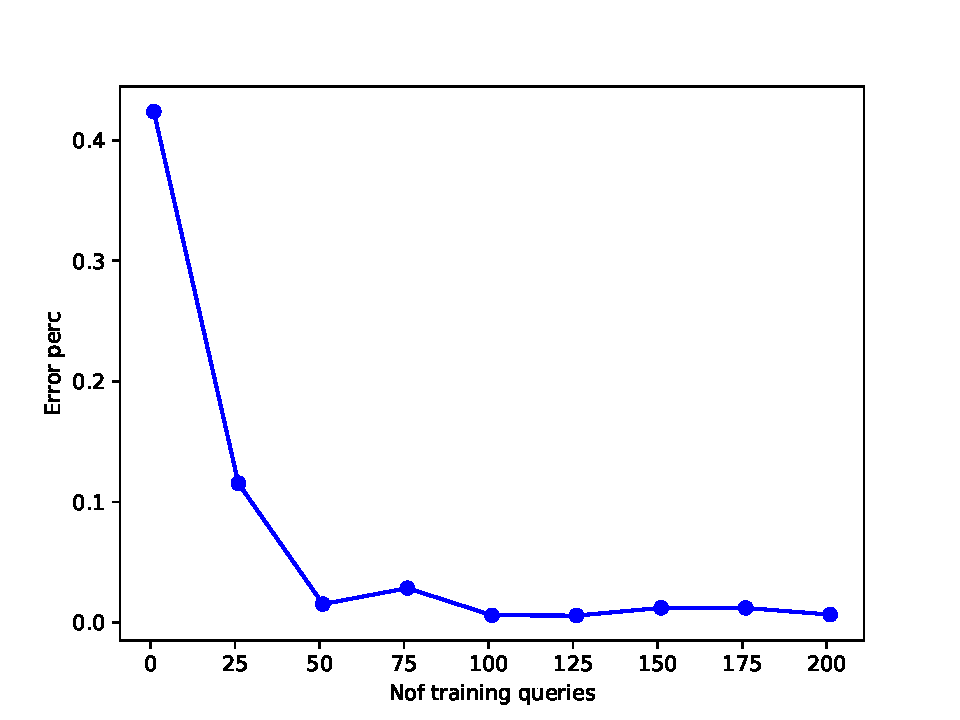
\includegraphics[scale=0.4]{figs/tpch10/tpch10_sel03_error.pdf}
     \caption{Query 03 select error}
     \label{fig:tpch_sel03}
   \end{subfigure}
   \begin{subfigure}[t]{0.5\textwidth}
     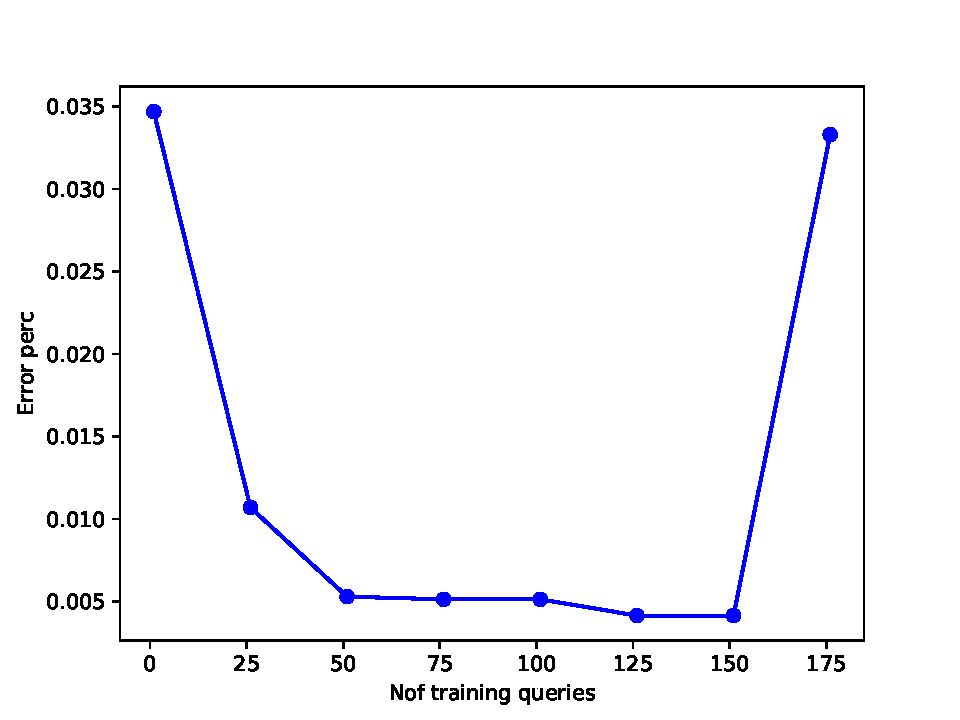
\includegraphics[scale=0.4]{figs/tpch10/tpch10_sel04_error.pdf}
     \caption{Query 04 select error}
     \label{fig:tpch_sel04}
    \end{subfigure}

    \begin{subfigure}[t]{0.5\textwidth}
      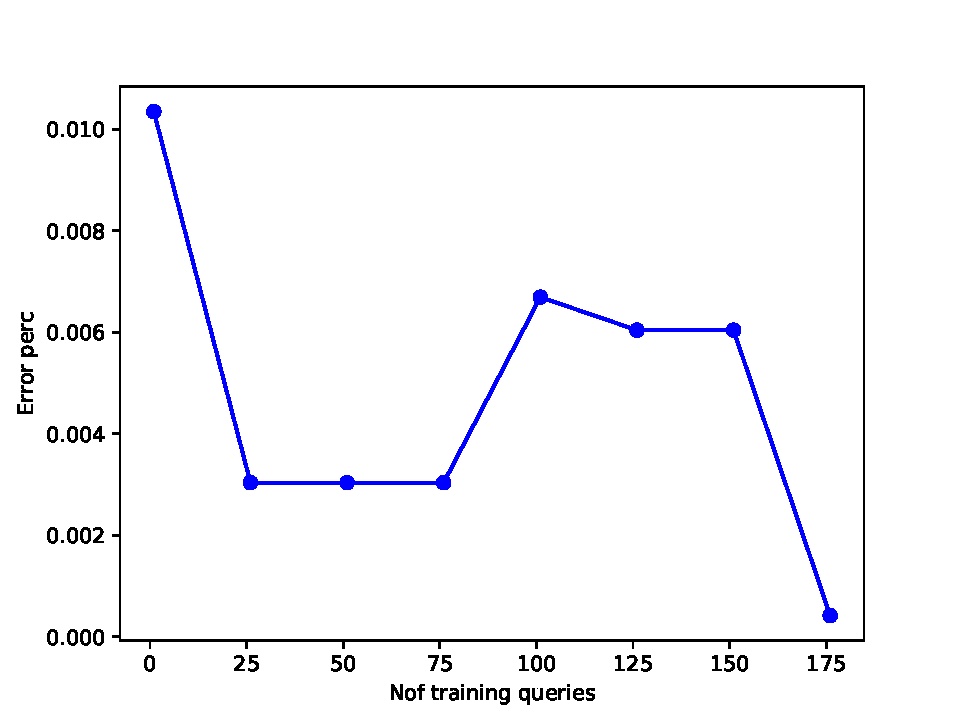
\includegraphics[scale=0.4]{figs/tpch10/tpch10_sel05_error.pdf}
      \caption{Query 05 select error}
      \label{fig:tpch_sel05}
    \end{subfigure}
    \begin{subfigure}[t]{0.5\textwidth}
      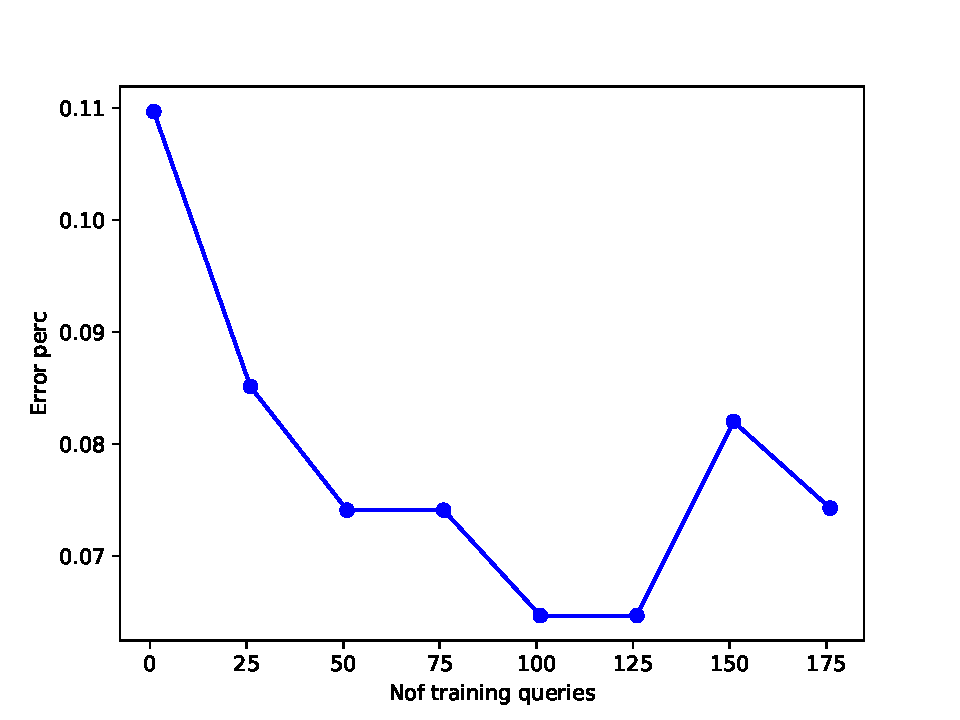
\includegraphics[scale=0.4]{figs/tpch10/tpch10_sel06_error.pdf}
      \caption{Query 06 select error}
      \label{fig:tpch_sel06}
     \end{subfigure}

     \begin{subfigure}[t]{0.5\textwidth}
       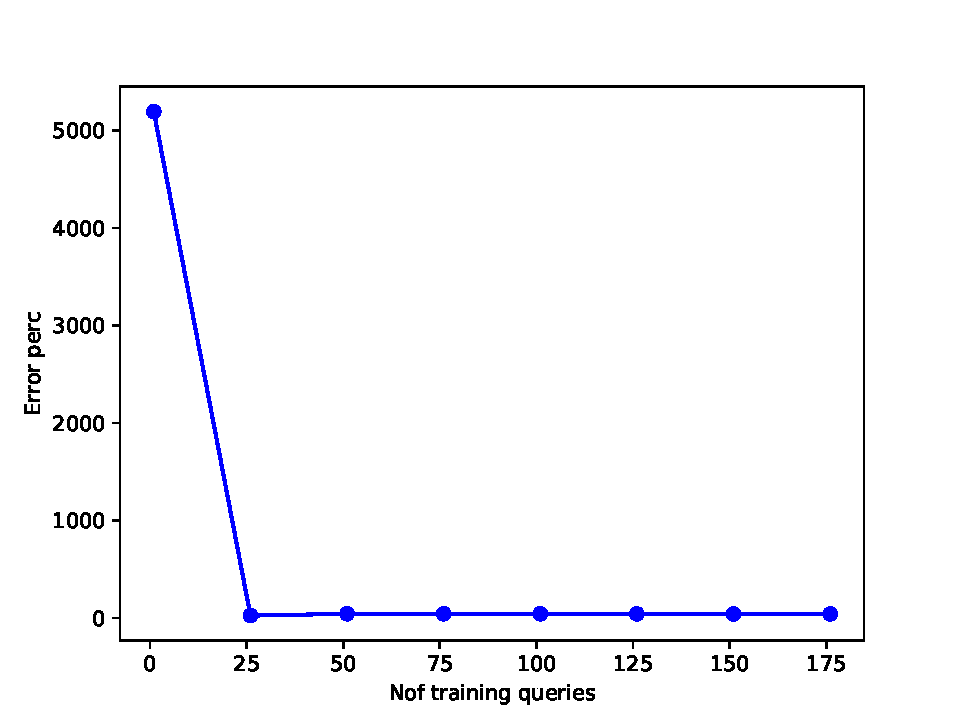
\includegraphics[scale=0.4]{figs/tpch10/tpch10_sel07_error.pdf}
       \caption{Query 07 select error}
       \label{fig:tpch_sel07}
     \end{subfigure}
     \begin{subfigure}[t]{0.5\textwidth}
       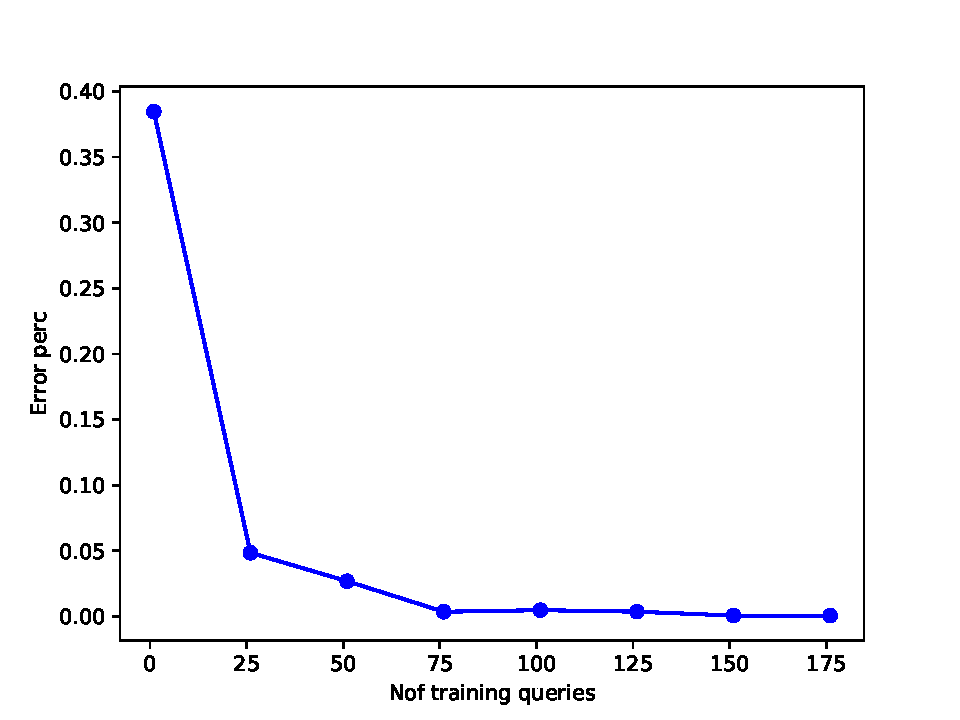
\includegraphics[scale=0.4]{figs/tpch10/tpch10_sel08_error.pdf}
       \caption{Query 08 select error}
       \label{fig:tpch_sel08}
      \end{subfigure}
\end{figure}

\begin{figure}[!htb]
  \begin{subfigure}[t]{0.5\textwidth}
    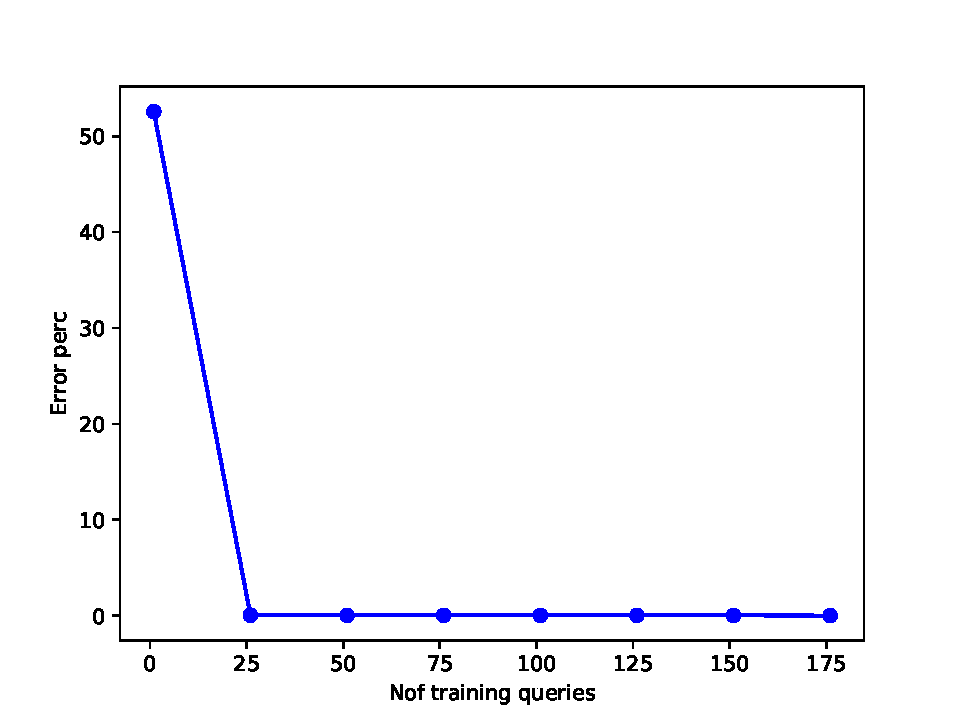
\includegraphics[scale=0.4]{figs/tpch10/tpch10_sel10_error.pdf}
    \caption{Query 10 select error}
    \label{fig:tpch_sel10}
  \end{subfigure}
  \begin{subfigure}[t]{0.5\textwidth}
    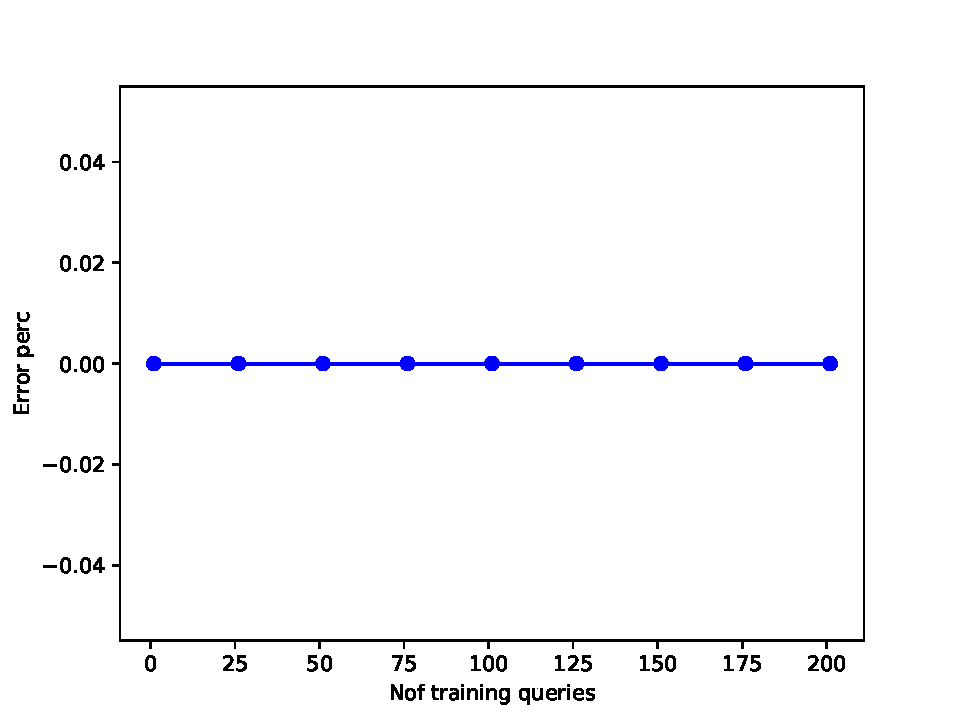
\includegraphics[scale=0.4]{figs/tpch10/tpch10_sel11_error.pdf}
    \caption{Query 11 select error}
    \label{fig:tpch_sel11}
   \end{subfigure}

   \begin{subfigure}[t]{0.5\textwidth}
     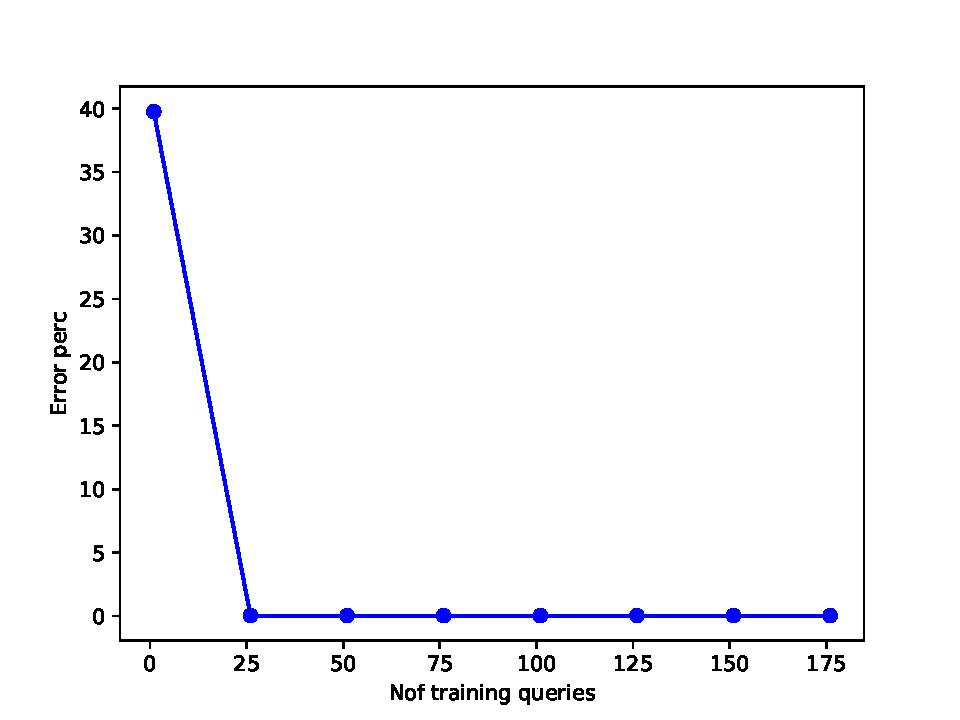
\includegraphics[scale=0.4]{figs/tpch10/tpch10_sel12_error.pdf}
     \caption{Query 12 select error}
     \label{fig:tpch_sel12}
   \end{subfigure}
   \begin{subfigure}[t]{0.5\textwidth}
     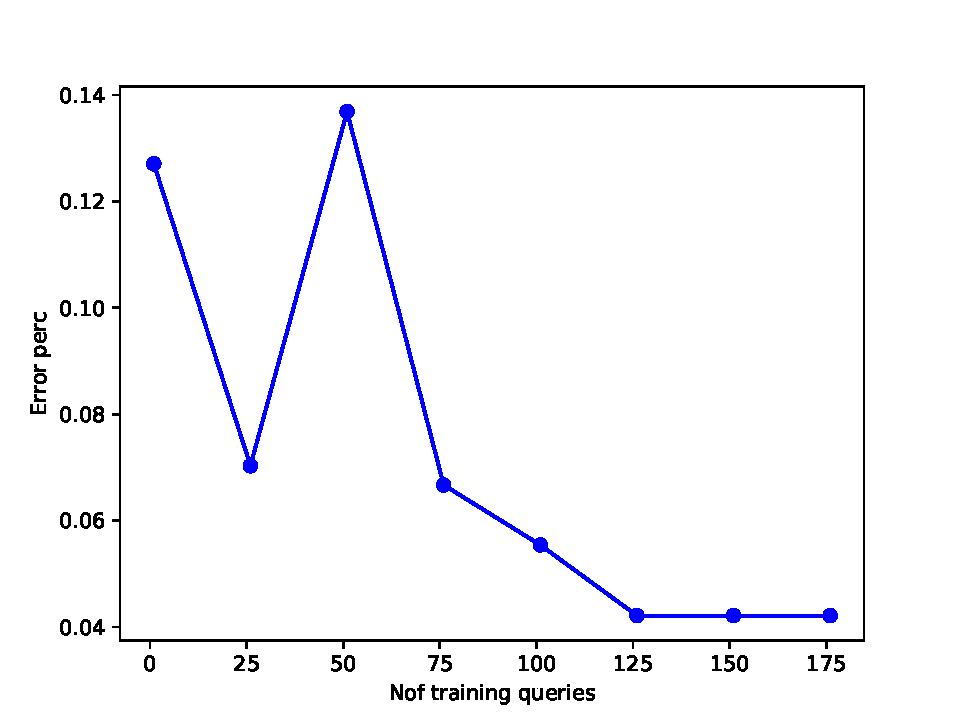
\includegraphics[scale=0.4]{figs/tpch10/tpch10_sel14_error.pdf}
     \caption{Query 14 select error}
     \label{fig:tpch_sel14}
    \end{subfigure}

    \begin{subfigure}[t]{0.5\textwidth}
      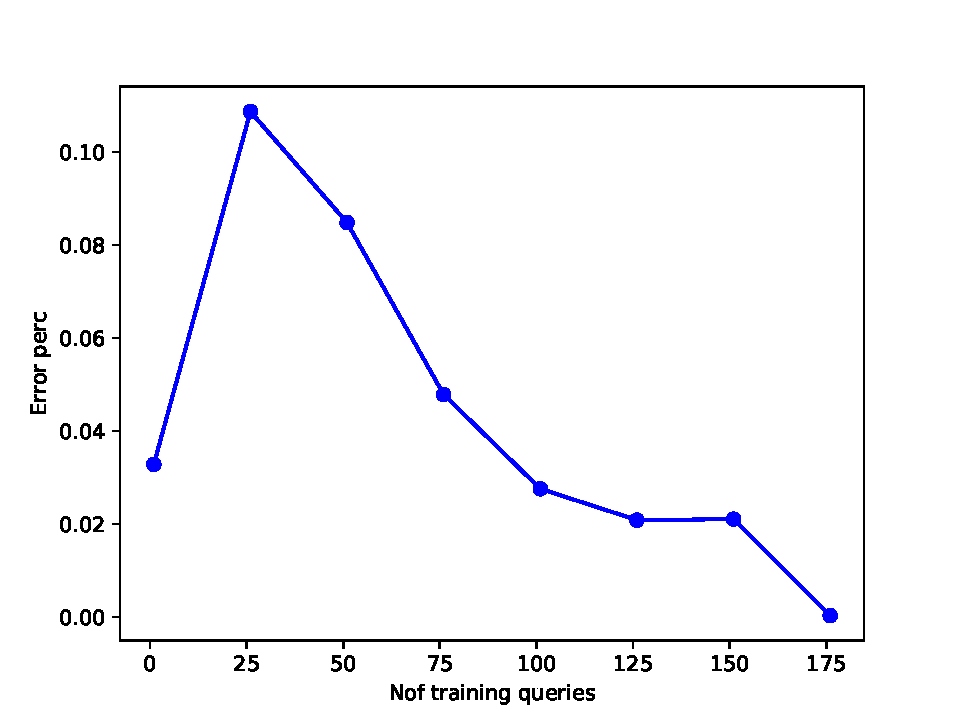
\includegraphics[scale=0.4]{figs/tpch10/tpch10_sel15_error.pdf}
      \caption{Query 15 select error}
      \label{fig:tpch_sel15}
    \end{subfigure}
    \begin{subfigure}[t]{0.5\textwidth}
      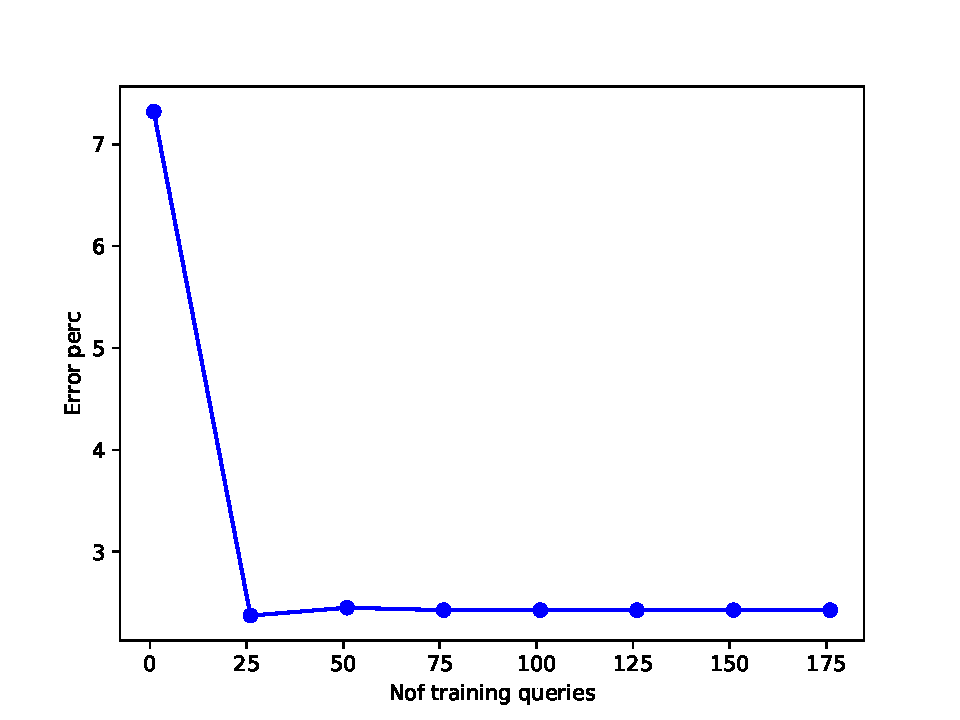
\includegraphics[scale=0.4]{figs/tpch10/tpch10_sel16_error.pdf}
      \caption{Query 16 select error}
      \label{fig:tpch_sel16}
     \end{subfigure}

     \begin{subfigure}[t]{0.5\textwidth}
       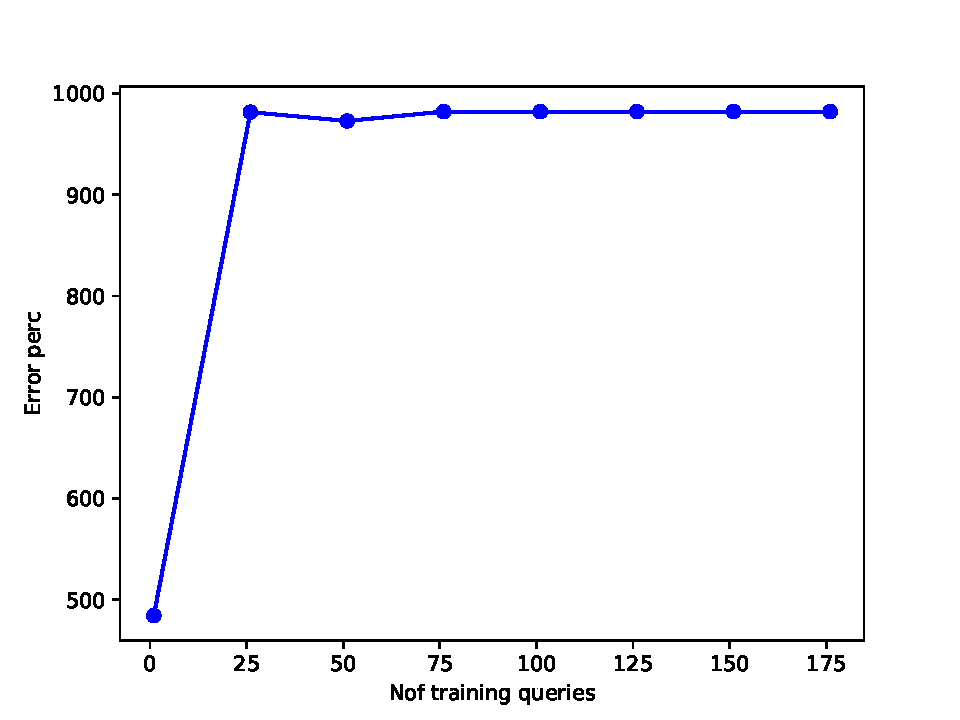
\includegraphics[scale=0.4]{figs/tpch10/tpch10_sel17_error.pdf}
       \caption{Query 17 select error}
       \label{fig:tpch_sel17}
     \end{subfigure}
     \begin{subfigure}[t]{0.5\textwidth}
       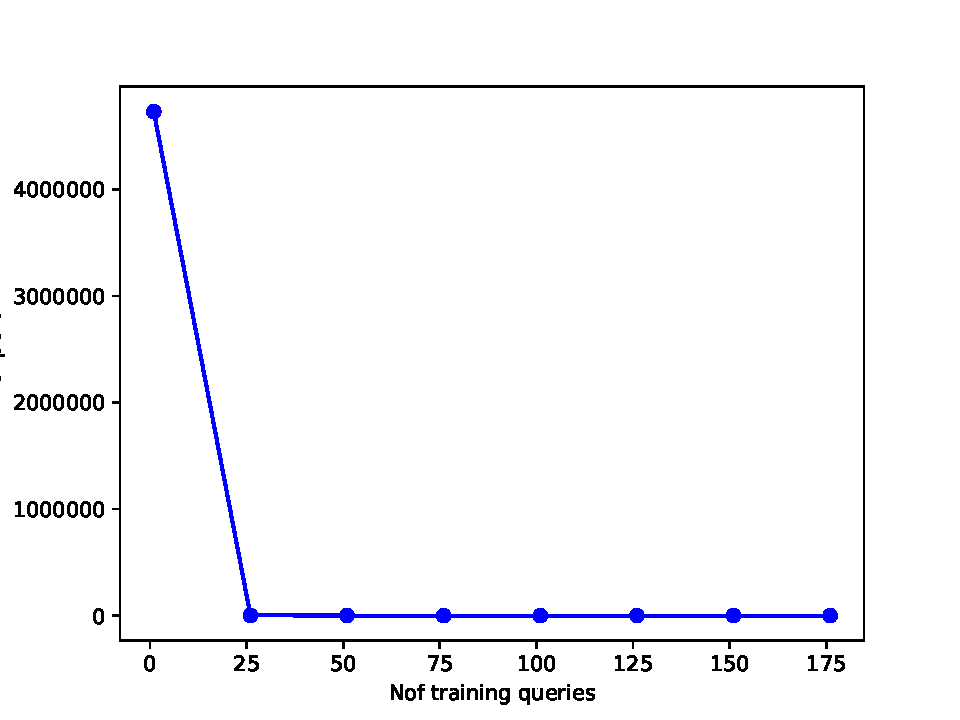
\includegraphics[scale=0.4]{figs/tpch10/tpch10_sel18_error.pdf}
       \caption{Query 18 select error}
       \label{fig:tpch_sel18}
      \end{subfigure}
\end{figure}

\begin{figure}[!htb]
    \begin{subfigure}[t]{0.5\textwidth}
      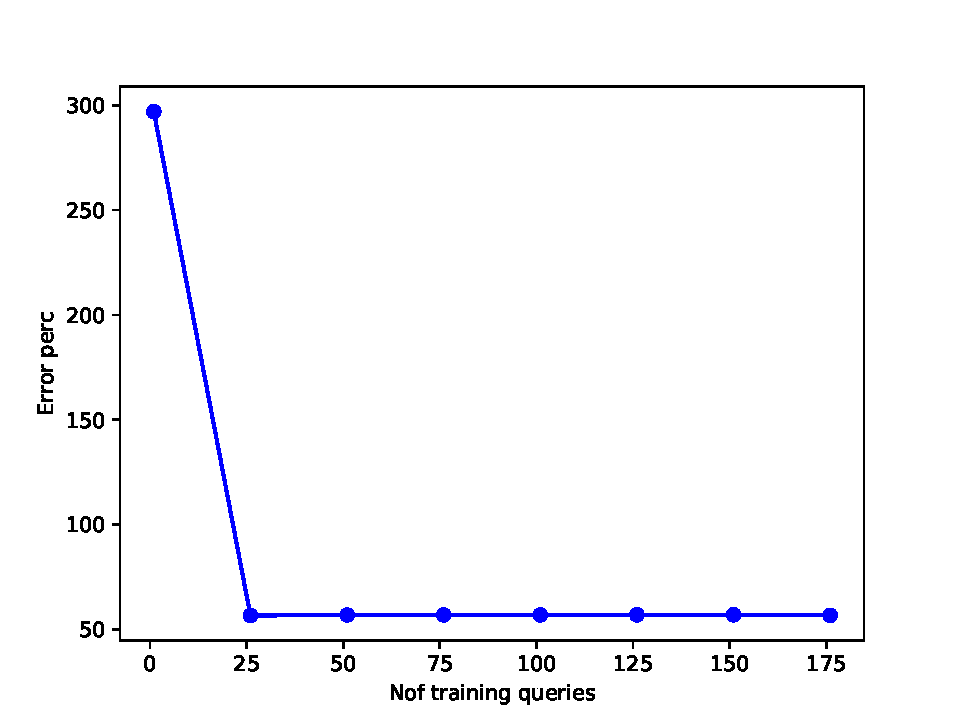
\includegraphics[scale=0.4]{figs/tpch10/tpch10_sel19_error.pdf}
      \caption{Query 19 select error}
      \label{fig:tpch_sel19}
    \end{subfigure}
    \begin{subfigure}[t]{0.5\textwidth}
      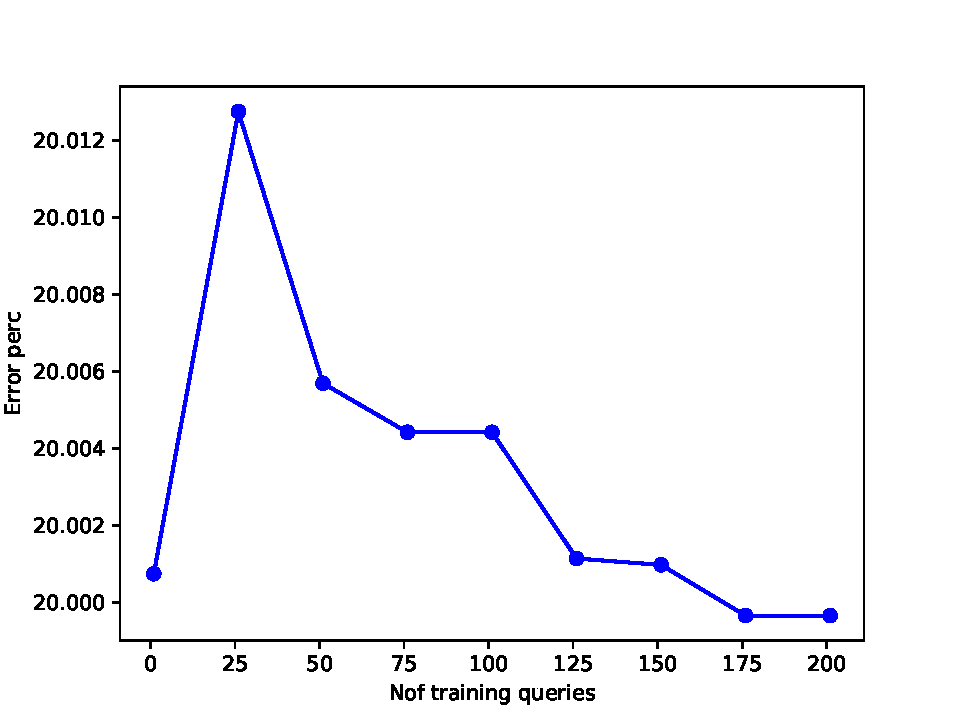
\includegraphics[scale=0.4]{figs/tpch10/tpch10_sel20_error.pdf}
      \caption{Query 20 select error}
      \label{fig:tpch_sel20}
     \end{subfigure}

     \begin{subfigure}[t]{0.5\textwidth}
       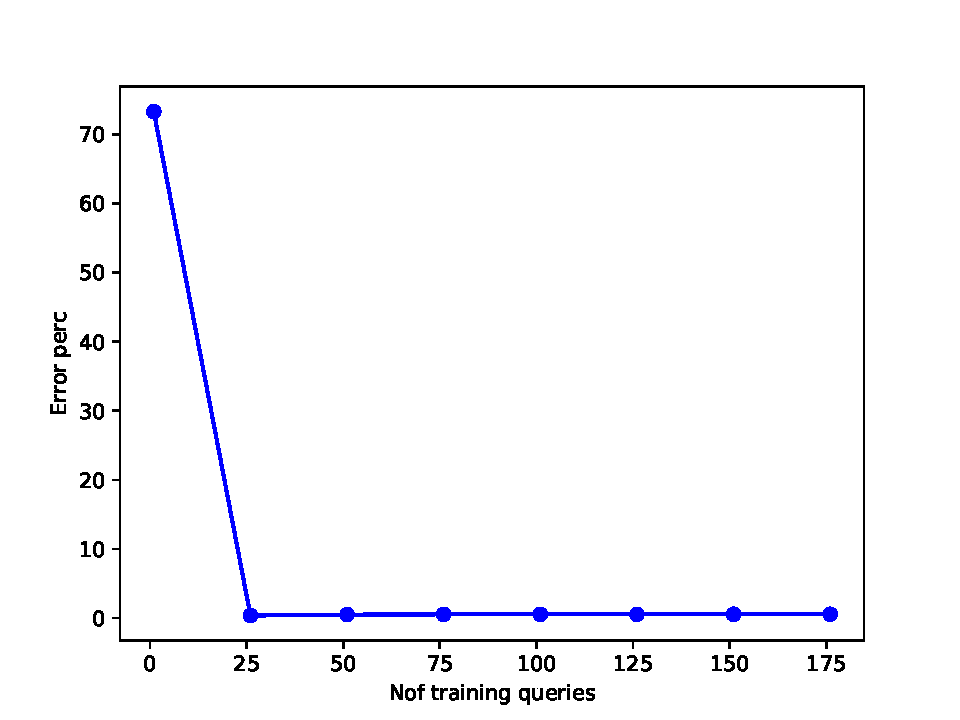
\includegraphics[scale=0.4]{figs/tpch10/tpch10_sel21_error.pdf}
       \caption{Query 21 select error}
       \label{fig:tpch_sel21}
     \end{subfigure}
     \begin{subfigure}[t]{0.5\textwidth}
       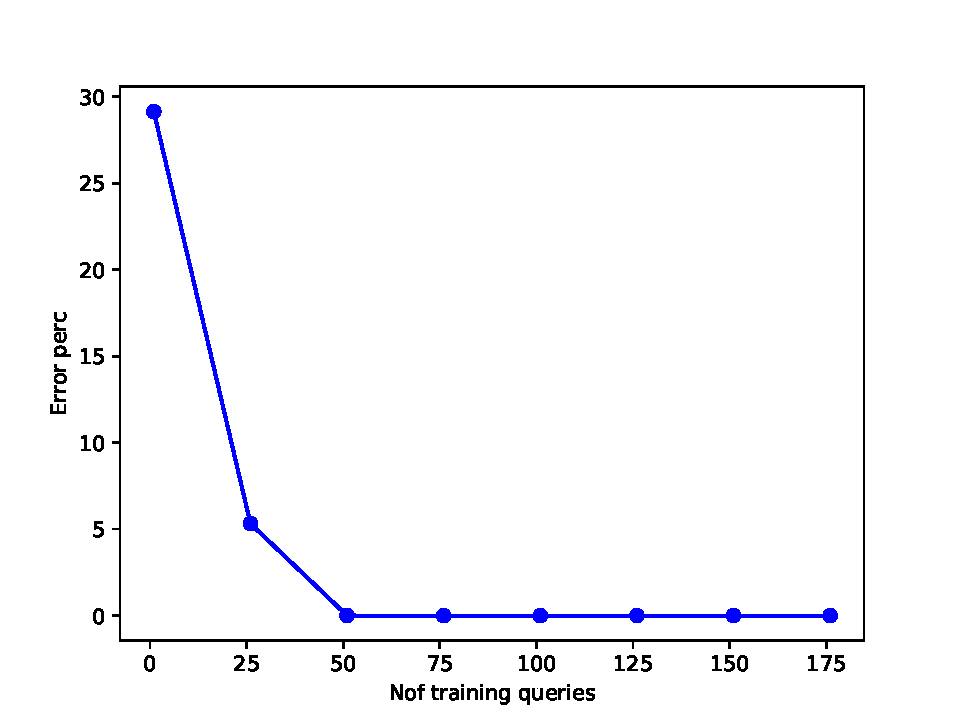
\includegraphics[scale=0.4]{figs/tpch10/tpch10_sel22_error.pdf}
       \caption{Query 22 select error}
       \label{fig:tpch_sel22}
      \end{subfigure}
\end{figure}


% \begin{figure}[!htb]
%   \begin{subfigure}[t]{0.5\textwidth}
%     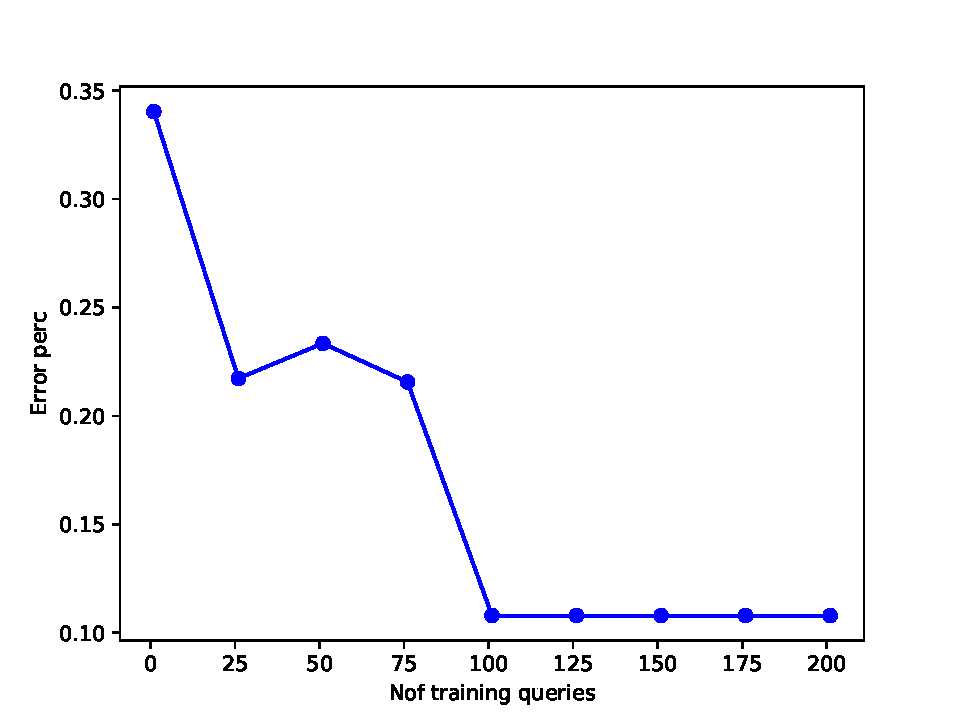
\includegraphics[scale=0.4]{figs/tpch10/tpch10_sel01_error.pdf}
%     \caption{Query 04 select error}
%     \label{fig:sel04}
%   \end{subfigure}
%   \begin{subfigure}[t]{0.5\textwidth}
%     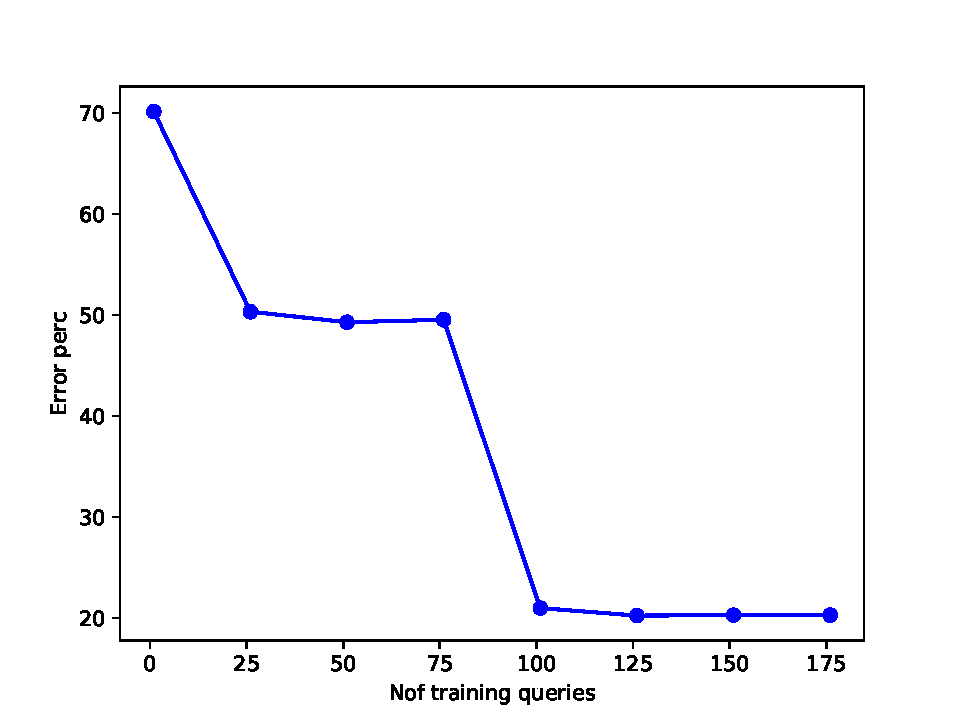
\includegraphics[scale=0.4]{figs/tpch10/tpch10_sel02_error.pdf}
%     \caption{Query 04 memory footprint}
%     \label{fig:mem04}
%    \end{subfigure}
% \end{figure}

\subsection{Airtraffic Queries}
%TODO some info about airtraffic...
As a training set for each query, we used 1000 versions of the
same query, randomized on the selection values. As a test set we used the original
query.
\subsubsection{Q04}
Query 4 (Figure \ref{sel:sql4}) selects all flights that have a departure delay greater than 15 minutes.
The training queries are randomized based on the DepDelay bound.
From the prediction perspective, this selection is interesting because
departure delay does not follow a uniform distribution(more like a normal),
thus is more challenging to accurately predict.
Figures  \ref{fig:sel04}, \ref{fig:mem04} show the error percentage for the
selection, and the whole query respectively. The x axis is the number of queries
used as a training set, and the y axis the error \%. The initial selection error
for is 500\%, but as we insert more instructions to the dictionary we get closer
to the initial range, and we are able to make an accurate prediction. After the
first 400 instructions, the error drops to (...)\%.
The per query memory error follows a similar pattern,
but the error is smaller because select instructions represent a relatively
small proportion of the overall query memory usage.

\begin{figure}[t]
\begin{lstlisting}
SELECT "DayOfWeek", COUNT(*) AS "Flights"
FROM ontime
WHERE "DepDelay" > 15
GROUP BY "DayOfWeek"
ORDER BY "DayOfWeek";
\end{lstlisting}
  \caption{Query 4}
  \label{sel:sql4}
\end{figure}


\begin{figure}[!htb]
  \begin{subfigure}[t]{0.5\textwidth}
    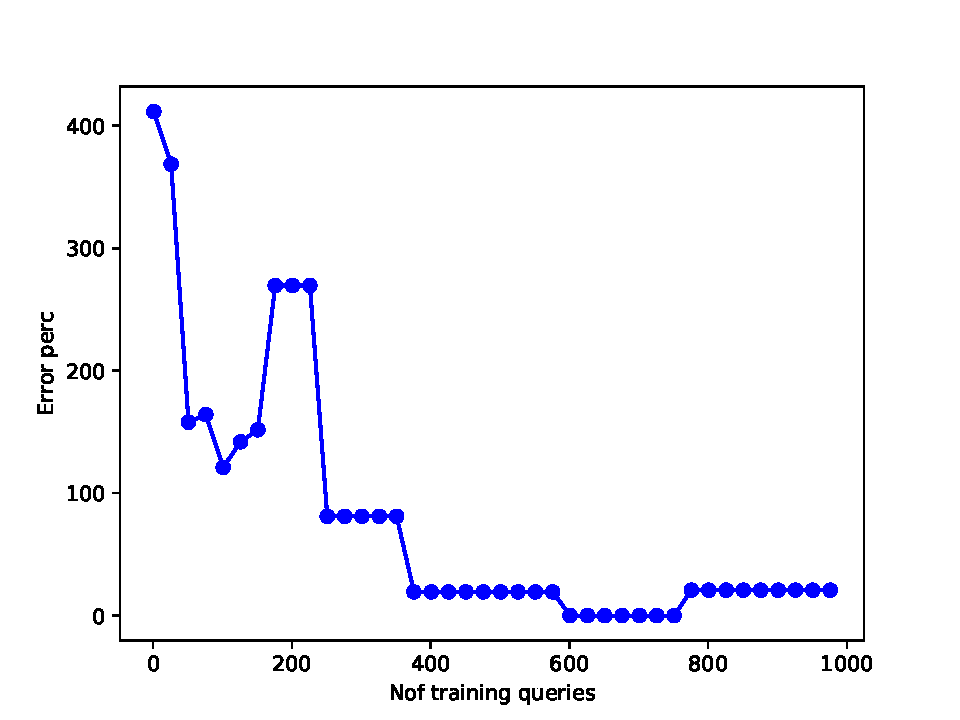
\includegraphics[scale=0.4]{figs/airtraffic/airtraffic_sel04_error.pdf}
    \caption{Query 04 select error}
    \label{fig:sel04}
  \end{subfigure}
  \begin{subfigure}[t]{0.5\textwidth}
    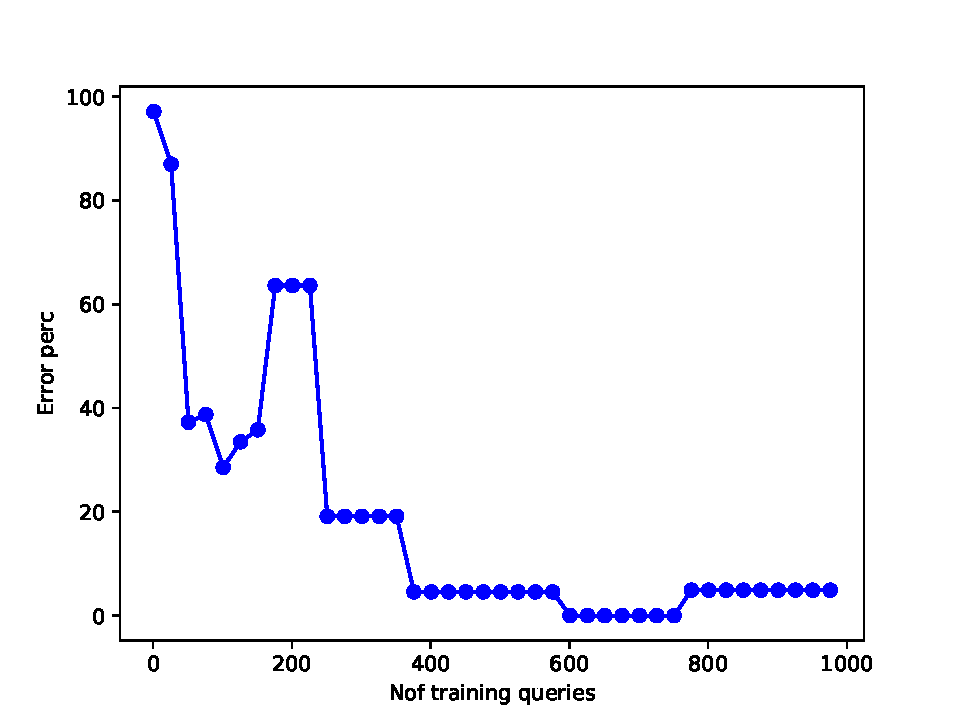
\includegraphics[scale=0.4]{figs/airtraffic/airtraffic_q04_memerror.pdf}
    \caption{Query 04 memory footprint}
    \label{fig:mem04}
   \end{subfigure}
\end{figure}

\subsubsection{Q09}

Query 9(Figure \ref{sel:sql09}) selects all flights on a specific date
for which the departure and the arrival delay are greater than 15 minutes.
The memory error(Figure \ref{fig:sel09}) is very small,
due to the very high selectivity of the query,
whereas the selection error(Figure \ref{fig:mem09}) seems to fluctuate a lot
betwwn 20 and 40\%. The reason we believe this is happening is that all three columns
(depdelay, arrdelay, date) are strongly correlated, making it very hard
for the prediction algorithm to converge.

\begin{figure}[!htb]
\begin{lstlisting}[frame=single]
WITH t1 AS (
    SELECT "Origin","CRSDepTime","DepDelay","Dest","ArrDelay","CRSArrTime"
    FROM ontime
    WHERE "DepDelay" > 15 AND "ArrDelay" > 15
      AND "Month" = 3 AND "DayofMonth" = 24 AND "Year" = 2013
)
SELECT t1."Origin" AS "Airport1",
  CAST(AVG(t1."DepDelay") AS DECIMAL(8,2)) AS "AVGDepDelay",
  CAST(AVG(t1."ArrDelay") AS DECIMAL(8,2)) AS "AVGArrDelay", t2."Origin" AS "Airport2",
  CAST(AVG(t2."DepDelay") AS DECIMAL(8,2)) AS "AVGDepDelay2",
  CAST(AVG(t2."ArrDelay") AS DECIMAL(8,2)) AS "AVGArrDelay2", t2."Dest" AS "Airport3"
FROM t1, t1 AS t2
WHERE t1."Dest" = t2."Origin" AND t1."CRSArrTime" < t2."CRSDepTime"
GROUP BY t1."Origin", t2."Origin", t2."Dest"
ORDER BY "AVGDepDelay" DESC,"AVGArrDelay" DESC,"AVGDepDelay2" DESC,"AVGArrDelay2" DESC
\end{lstlisting}
  \caption{Query 09}
  \label{sel:sql09}
\end{figure}

\begin{figure}[!htb]
  \begin{subfigure}[t]{0.5\textwidth}
    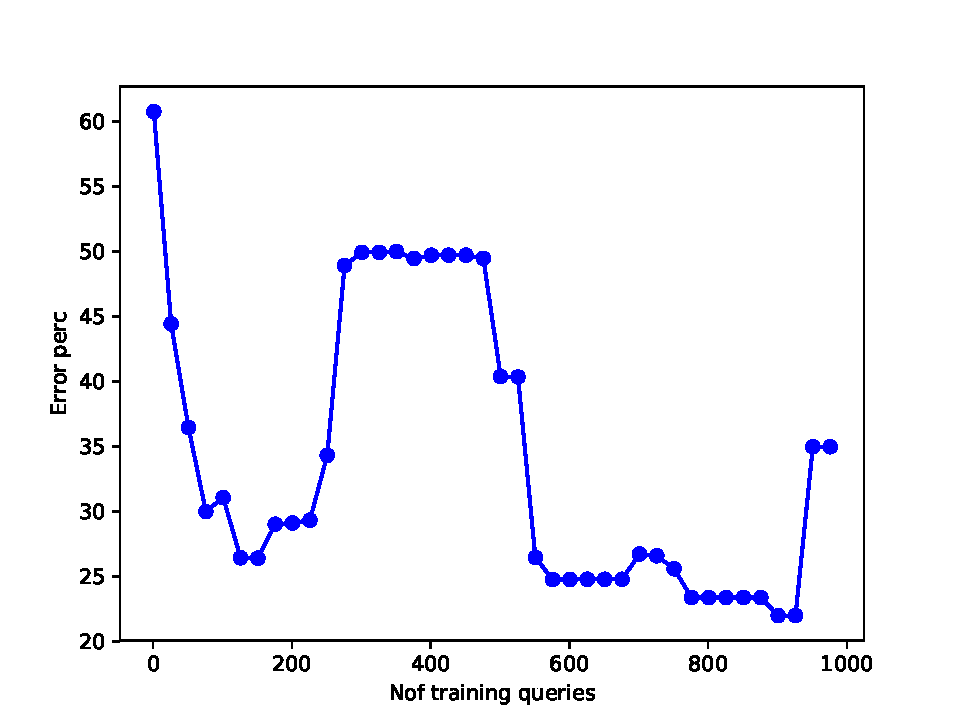
\includegraphics[scale=0.4]{figs/airtraffic/airtraffic_sel09_error.pdf}
    \caption{Query 09 select error}
    \label{fig:sel09}
  \end{subfigure}
  \begin{subfigure}[t]{0.5\textwidth}
    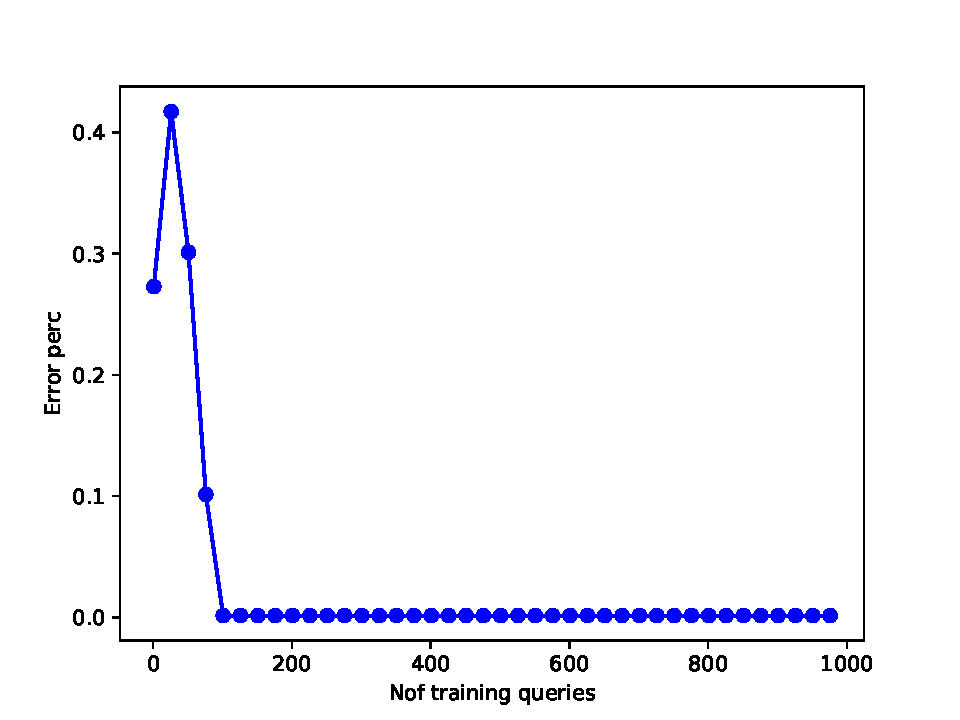
\includegraphics[scale=0.4]{figs/airtraffic/airtraffic_q09_memerror.pdf}
    \caption{Query 09 memory footprint}
    \label{fig:mem09}
   \end{subfigure}
\end{figure}

\subsubsection{Q10}

Query 10(Figure \ref{sel:sql10}) contains two point selections,
regarding the origin and the destination of the flight. Figures \ref{fig:sel10}
and \ref{fig:mem10} show the selection and memory error. The selection error
starts at 100\% for 1 query, dropping gradually to almost 0 as we insert more
instructions. The memory error follows a similar pattern from 6.5\% to 0\%.
The reason for this behaviour is that the distribution of the
Carrier column points is not uniform, thus we cannot make accurate estimations
for one point based on another point. By inserting more instructions to the
training set, after a while we memorize the exact point, so the error converges
to zero. In the future we plan to incorporate histogram information
to overcome those problems.


\begin{figure}[htb!]
\begin{lstlisting}[frame=single]
ITH t1 AS ( -- flights to ORD
    SELECT "Origin" AS ap, COUNT(*) AS cnt_in
    FROM ontime
    WHERE "Dest" = 'ORD'
    GROUP BY "Origin"
),
t2 AS ( -- flights from ORD
    SELECT "Dest" AS ap, COUNT(*) AS cnt_out
    FROM ontime
    WHERE "Origin" = 'ORD'
    GROUP BY "Dest"
),
t3 AS ( -- merge t1, t2 into one table
    SELECT t1.ap AS ap1, t1.cnt_in, t2.ap AS ap2, t2.cnt_out
    FROM t1 FULL OUTER JOIN t2 ON (t1.ap = t2.ap))
SELECT CASE WHEN ap1 IS NULL THEN ap2 ELSE ap1 END AS "Airport",
       cnt_in AS "InboundFlights", cnt_out AS "OutboundFlights"
FROM t3;
\end{lstlisting}
  \caption{Query 10}
  \label{sel:sql10}
\end{figure}

\begin{figure}[htb!]
  \begin{subfigure}[t]{0.5\textwidth}
    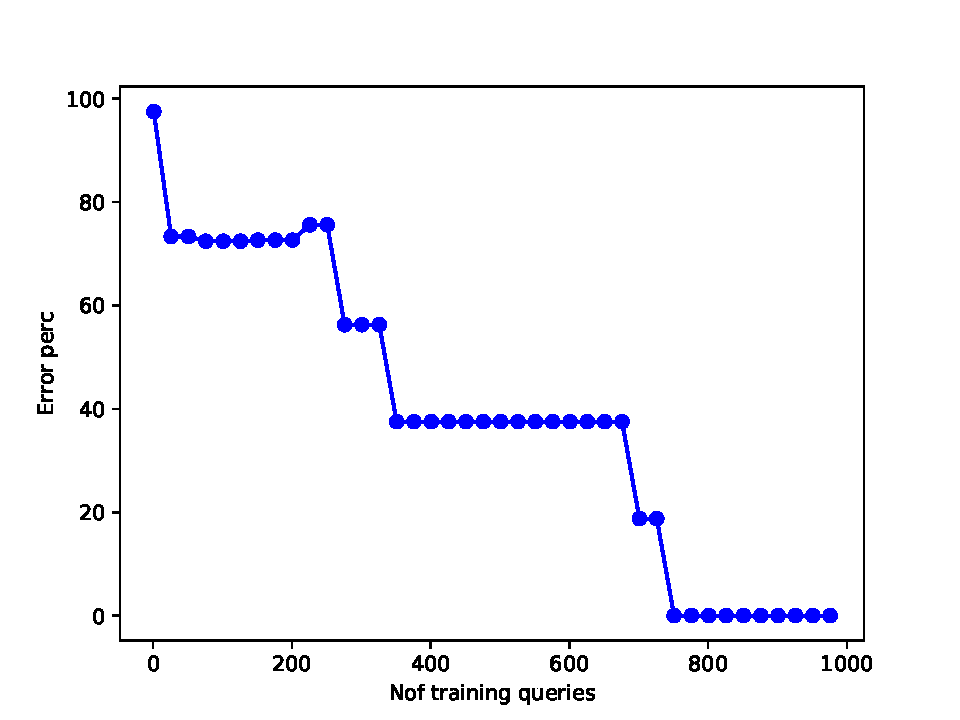
\includegraphics[scale=0.4]{figs/airtraffic/airtraffic_sel10_error.pdf}
    \caption{Query 10 select error}
    \label{fig:sel10}
  \end{subfigure}
  \begin{subfigure}[t]{0.5\textwidth}
    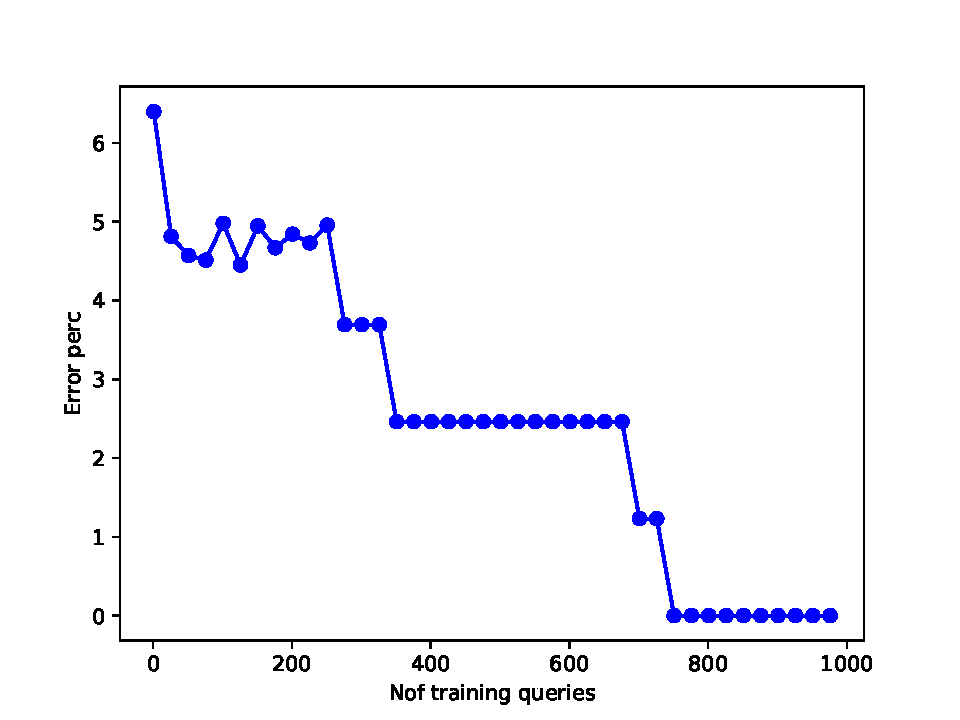
\includegraphics[scale=0.4]{figs/airtraffic/airtraffic_q10_memerror.pdf}
    \caption{Query 10 memory footprint}
    \label{fig:mem10}
   \end{subfigure}
\end{figure}


\subsubsection{Q11}

Query 11 detects differences in flight reservations before and after 9/11.
The selection column is the FlightDate, and the query contains two range
selections. We randomized the lower and upper bound of both selections in the
training set. Figures \ref{fig:sel11} and \ref{fig:mem11} show the selection and memory error.
The initial selection error is 400\% with a memory footprint error
of 16\%. Again the memory footprint error is much smaller than the selection error
due to the selectivity of the query. After the first 100 training queries,
we get close enough to the range of the test query,
so the error is stabilized between 3-20\% till the end.

\begin{figure}[htb!]
\begin{lstlisting}[frame=single]
WITH t1 AS ( -- #flights per route before 9/11
    SELECT SQL_MIN("Origin", "Dest") || ' <-> ' ||
           SQL_MAX("Origin", "Dest") AS route,
           COUNT(*) AS cnt_before
    FROM ontime
    WHERE '2010-09-11' < "FlightDate" AND "FlightDate" < '2011-09-11'
    GROUP BY route
),
t2 AS ( -- #flights per route after 8/11
    SELECT SQL_MIN("Origin", "Dest") || ' <-> ' ||
           SQL_MAX("Origin", "Dest") AS route,
           COUNT(*) AS cnt_after
    FROM ontime
    WHERE '2011-09-11' <= "FlightDate" AND "FlightDate" < '2012-09-11'
    GROUP BY route
),
t3 AS ( -- merge t1, t2 into one table
    SELECT t1.route AS route1, t1.cnt_before, t2.route AS route2, t2.cnt_after
    FROM t1 FULL OUTER JOIN t2 ON (t1.route = t2.route)
)
SELECT CASE WHEN route1 IS NULL THEN route2 ELSE route1 END AS "Route",
       cnt_before AS "FlightsBefore", cnt_after AS "FlightsAfter"
FROM t3;
\end{lstlisting}
  \caption{Query 11}
  \label{sel:sql11}
\end{figure}

\begin{figure}[htb!]
 \begin{subfigure}[t]{0.5\textwidth}
   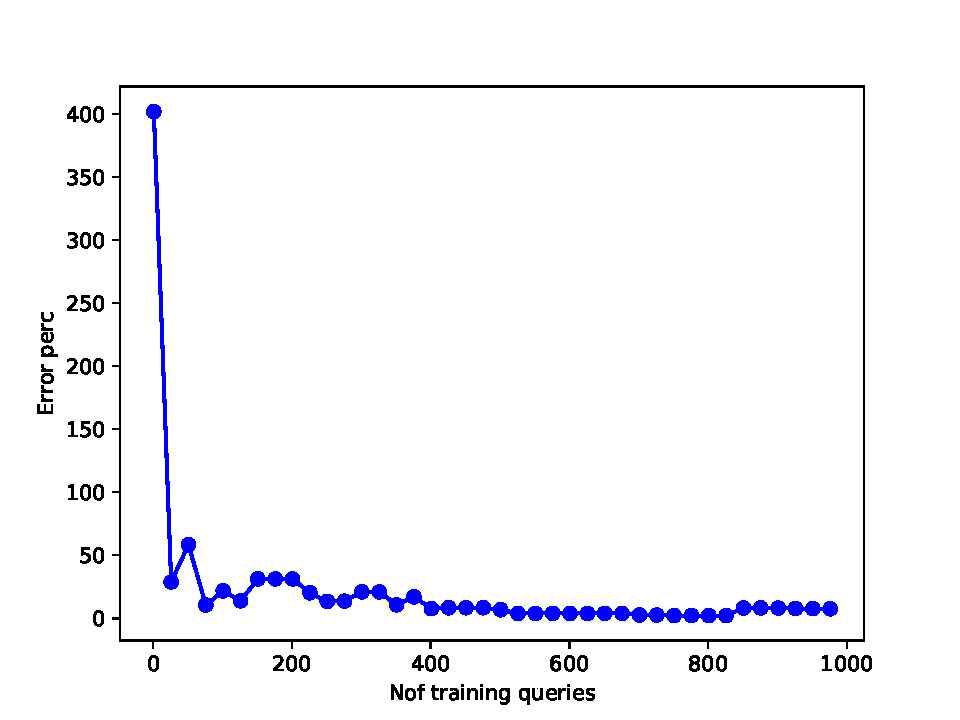
\includegraphics[scale=0.4]{figs/airtraffic/airtraffic_sel11_error.pdf}
   \caption{Query 11 select error}
   \label{fig:sel11}
 \end{subfigure}
 \begin{subfigure}[t]{0.5\textwidth}
   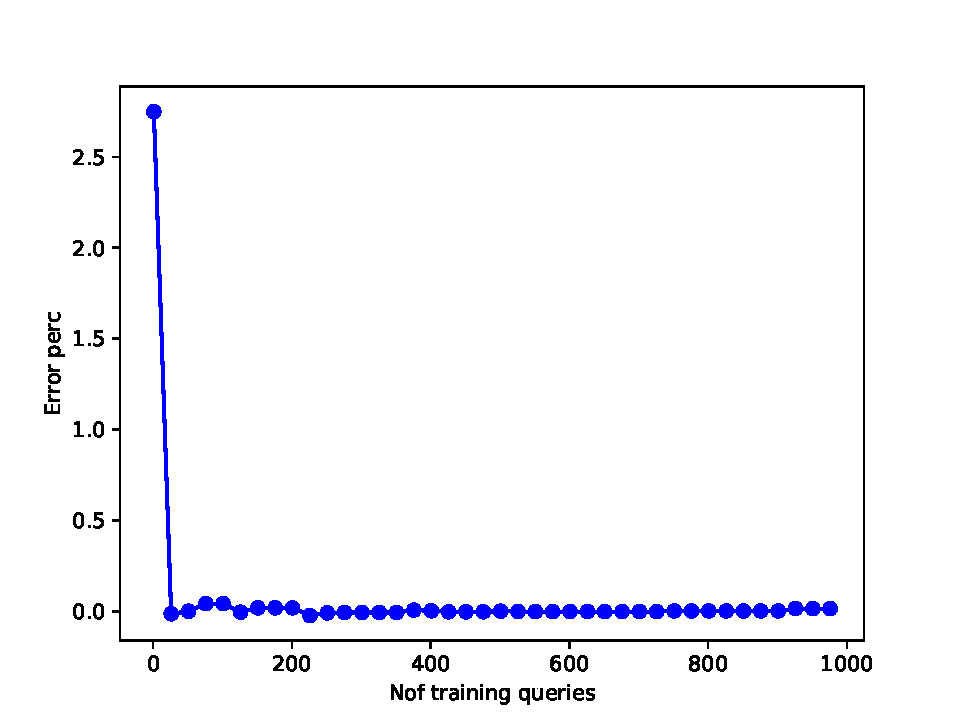
\includegraphics[scale=0.4]{figs/airtraffic/airtraffic_q11_memerror.pdf}
   \caption{Query 11 memory footprint}
   \label{fig:mem11}
  \end{subfigure}

\end{figure}


\subsubsection{Q15}

Query 15 does a point selection on the Carrier column (string).
Figures \ref{fig:sel15} and \ref{fig:mem15} show the selection and memory error.
The carrier column is not uniformly distributed. As a result we cannot infer the
selectivity based on different points. This results to an initial large error
for the first 225 instructions, fluctuating from a 30 to a 70\% selection error.
As soon as we insert the exact point in the training set, the error drops to 0.

\begin{figure}[htb!]
\begin{lstlisting}[frame=single]
WITH t1 AS (
    SELECT "Carrier", CAST (FLOOR("CRSDepTime"%2400/100) AS INT) AS "Hour",
           CAST(AVG("ArrDelay") AS DECIMAL(8,2)) AS "PredictedArrDelay"
    FROM ontime
    WHERE Carrier = 'EA'
    GROUP BY "Carrier", "Hour"
),
t2 AS (
    SELECT t."Carrier", tmp.*
    FROM tmp, (SELECT DISTINCT "Carrier" FROM t1) AS t
)
SELECT "Carrier", "Hour", SUM("PredictedArrDelay")
FROM (SELECT * FROM t1 UNION SELECT * FROM t2) AS t
GROUP BY "Carrier", "Hour"
ORDER BY "Carrier", "Hour";
\end{lstlisting}
  \caption{Query 15}
  \label{sel:sql15}
\end{figure}


\begin{figure}[htb!]
  \begin{subfigure}[t]{0.5\textwidth}
    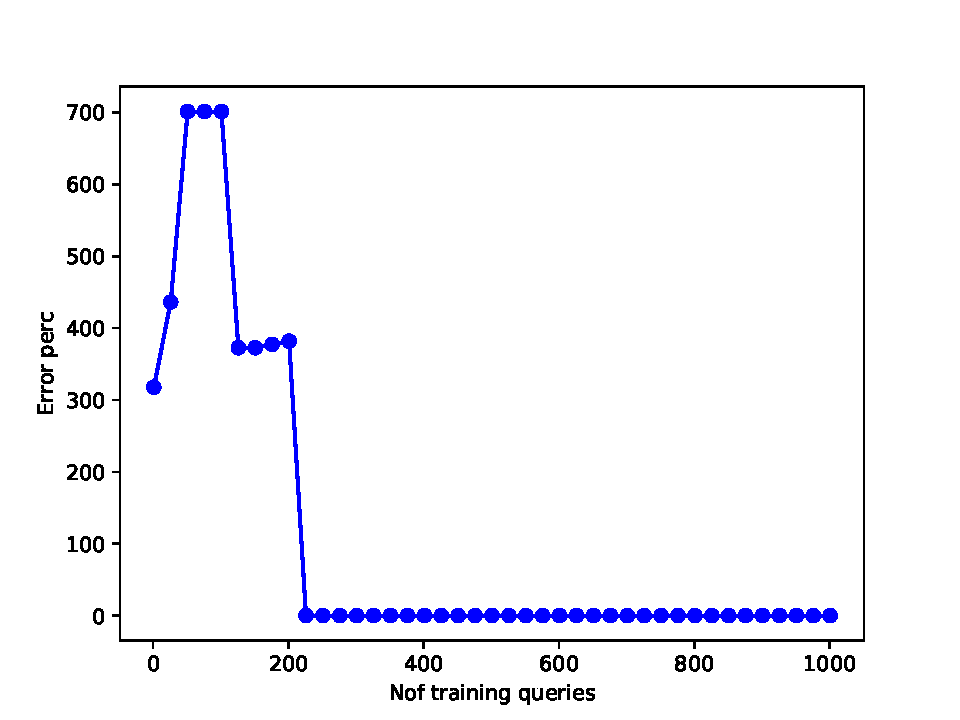
\includegraphics[scale=0.4]{figs/airtraffic/airtraffic_sel15_1_error.pdf}
    \caption{Query 15 select error}
    \label{fig:sel15}
  \end{subfigure}
  \begin{subfigure}[t]{0.5\textwidth}
    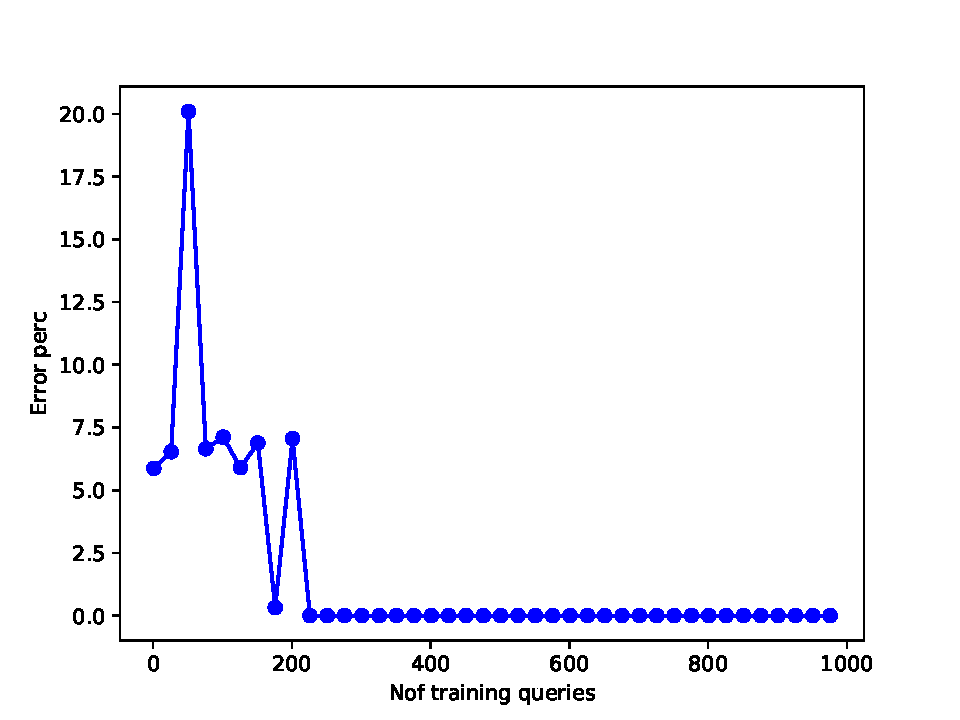
\includegraphics[scale=0.4]{figs/airtraffic/airtraffic_q15_1_memerror.pdf}
    \caption{Query 15 memory footprint}
    \label{fig:mem15}
   \end{subfigure}

\end{figure}

\subsubsection{Q19}
Query 19 like query 15 performs a selection on the Carrier column, thus
the selection error graph is very similar to query 15. The memory error
follows a similar pattern as query 15, but is smaller because query 19 uses
more columns, thus more initial memory.
Figures \ref{fig:sel19} and \ref{fig:mem19} show the selection and memory error.

\begin{figure}[htb!]
\begin{lstlisting}[frame=single]
SELECT CAST (FLOOR("CRSDepTime"%2400/100) AS INT) AS "Hour",
       "Origin", "Dest", "Carrier",
       CAST(SUM("DepDel15") AS DOUBLE)/COUNT(*) >= 0.5 AS "PossibleLongDelay"
FROM ontime
WHERE Carrier = 'EV'
GROUP BY "Origin", "Dest", "Carrier", "Hour"
ORDER BY "PossibleLongDelay", "Hour", "Origin", "Dest", "Carrier";
\end{lstlisting}
  \caption{Query 19}
  \label{sel:sql19}
\end{figure}


\begin{figure}[t!]
  \begin{subfigure}[t]{0.5\textwidth}
    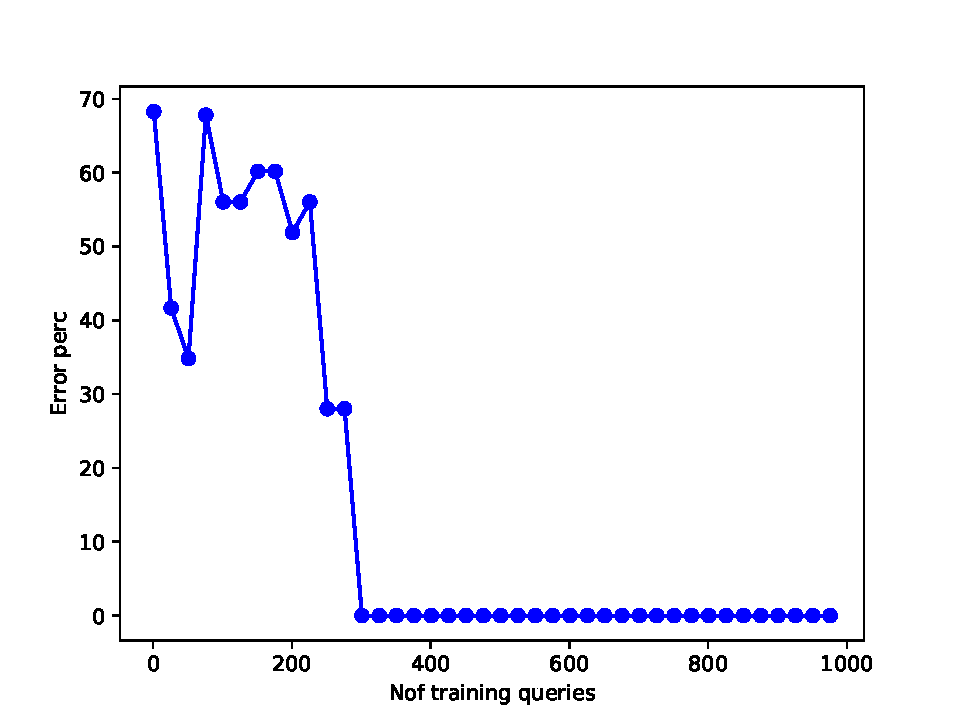
\includegraphics[scale=0.4]{figs/airtraffic/airtraffic_sel19_1_error.pdf}
    \caption{Query 19 select error}
    \label{fig:sel19}
  \end{subfigure}
  \begin{subfigure}[t]{0.5\textwidth}
    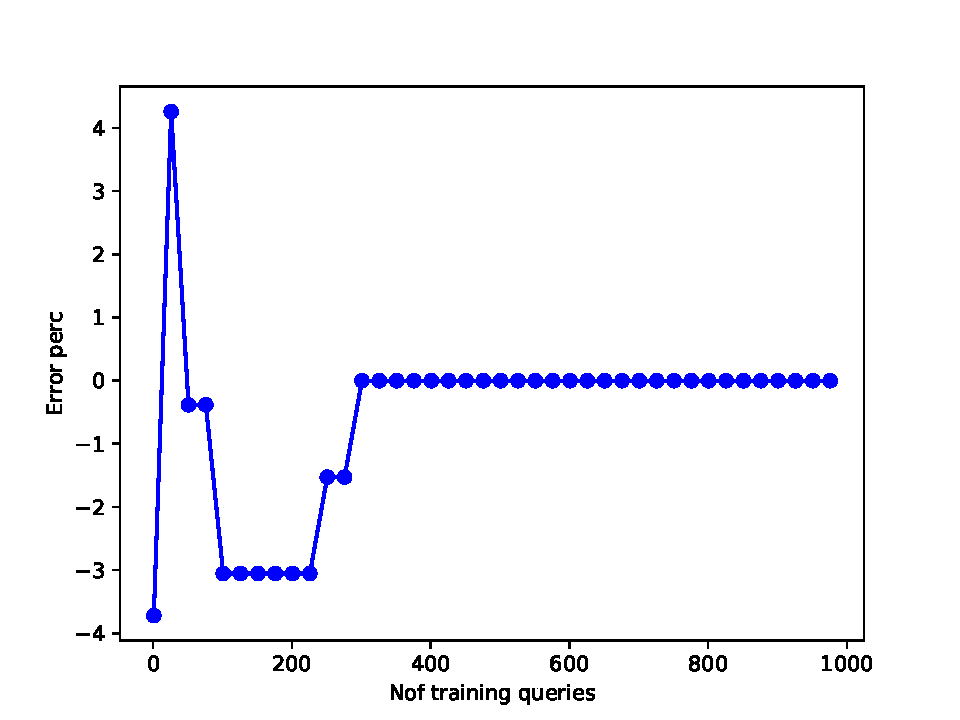
\includegraphics[scale=0.4]{figs/airtraffic/airtraffic_q19_1_memerror.pdf}
    \caption{Query 19 memory footprint}
    \label{fig:mem19}
   \end{subfigure}

\end{figure}



% \begin{figure}[ht]
%   \centering
%   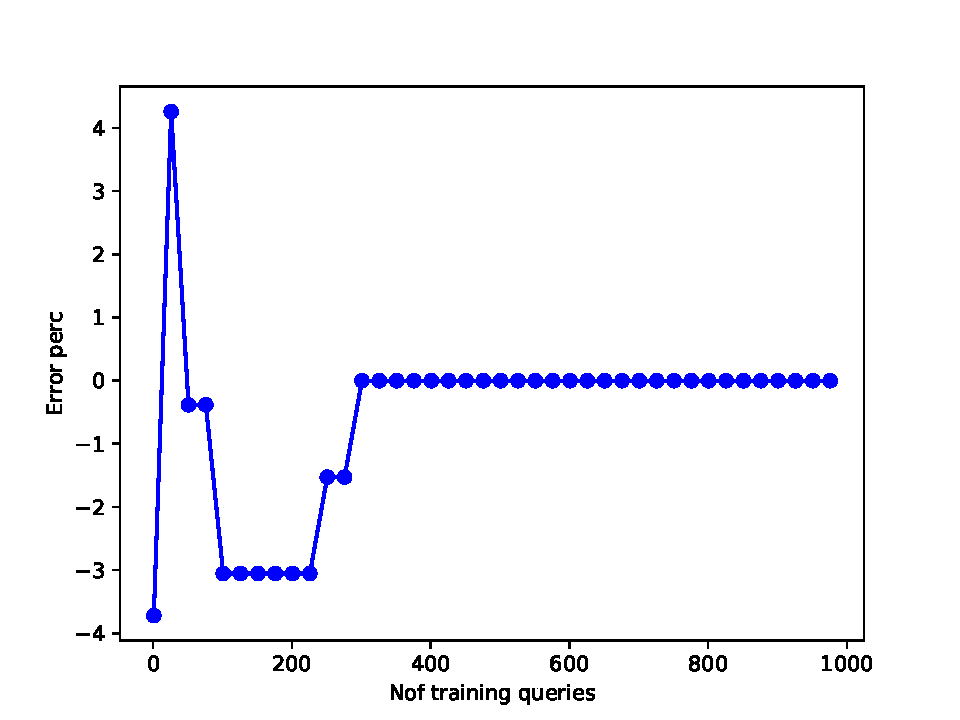
\includegraphics[scale=0.7]{figs/airtraffic/airtraffic_q19_1_memerror.pdf}
%   \caption{Query 4 memory footprint}
%   \label{fig:sel6}
% \end{figure}

%todo list query


\end{document}
